\section{QC Background}
\label{sec:swapping_background}

\para{Qubit States.}
Quantum computation manipulates \emph{qubits}
analogous to how classical computation manipulates \emph{bits}.  
At any given time, a bit may be in one of two states, traditionally represented by $0$
and $1$.  A quantum state represented by a
\emph{qubit} is a \emph{superposition} of classical
states, and is usually written as $\alpha_0\ket{0} + \alpha_1\ket{1}$,
where $\alpha_0$ and $\alpha_1$ are \emph{amplitudes} represented by
complex numbers and such that $\norm{\alpha_0}^2 + \norm{\alpha_1}^2 = 1$.
%%%%%%%%%%%%%%%%%%%%
Here, $\ket{0}$ and $\ket{1}$ are the standard (orthonormal) 
\emph{basis} states; concretely, they
may represent physical properties such as spin (down/up),
polarization, charge direction, etc.
%%%%%%%%
When a qubit such as above is \textit{measured}, it collapses to a 
$\ket{0}$ state with a probability of $\norm{\alpha_0}^2$ and to
a $\ket{1}$ state with a probability of $\norm{\alpha_1}^2$.
%%%%%%%%%%%%%%%%%%%%%
% Representation
%A state of a $2$-qubit  quantum system can be represented as 
%$\alpha_{00}\ket{00} + \alpha_{01}\ket{01} + \alpha_{10}\ket{10} +
%\alpha_{11}\ket{11}$, and 
In general, a state of an $n$ qubit
system can be represented as $\Sigma_{i=0}^{2^n-1} \alpha_i\ket{i}$
 where ``$i$'' in $\ket{i}$ is $i$'s bit representation. 
\eat{($\Sigma_{i=0}^{2^n-1}\norm{\alpha_i}^2=1$)}
Qubit mapping refers to the problem of assigning logical qubits used in quantum algorithms
to the physical qubits available on a quantum computer.
~\cite{yuwei2023exploit} exploits the regular structure of modern quantum architecture 
and~\cite{yuwei2023QFT} leverages technical intuition (i.e., educated guess) to advance qubit mapping in domain specific problems.

\para{Entanglement.}
Entangled pure\footnote{\tqbl{In this chapter, we largely deal with only
pure qubit states. Entanglement of general mixed states is defined in
terms of separation of density matrices~\cite{qd-2009}.}}
states are multi-qubit states that cannot be
"factorized" into independent single-qubit states.
E.g., the 
$2$-qubit state $\frac{1}{\sqrt{2}}\ket{00}
+ \frac{1}{\sqrt{2}}\ket{11}$; this particular system is a
\emph{maximally-entangled} state. 
We refer to maximally-entangled pairs of qubits as \epss.
%%%%%%%%%%%%%%%%%%
The surprising aspect of entangled states is that the combined
system continues to stay entangled, even when 
the individual qubits are physically separated by large distances.
This facilitates many applications, e.g., teleportation of qubit
states by local operations and classical information exchange, as
described next.

% Quantum data cannot be \emph{cloned}~\cite{wooterszurek-nocloning,Dieks-nocloning}, i.e., it is not possible to make \emph{independent} copies of arbitrary quantum information.  
% Consequently, direct transmission of quantum data 
% is subject to unrecoverable errors, 
% as classical procedures such as amplified signals 
% or re-transmission cannot be applied.
\para{Teleportation.} 
Direct transmission of quantum data 
is subject to unrecoverable errors, 
as classical procedures such as amplified signals 
or re-transmission cannot be applied due to quantum no-cloning~\cite{wooterszurek-nocloning,Dieks-nocloning}.\footnote{\tqbl{Quantum error
correction mechanisms~\cite{muralidharan2016optimal, Devitt_2013} can be used to mitigate the transmission errors, 
but their implementation is very challenging and is not expected to be used
until later generations of quantum networks.}}
%%%%%%%%%%%%%%%%%%%%%%%%%
An alternative mechanism
for quantum communication is \emph{teleportation}, Fig.~\ref{fig:swapping_teleport_swap} (a), where a qubit $q$ from a node $A$
is recreated in another node $B$ (\emph{while ``destroying'' the original
qubit $q$}) using only classical communication.
However, this process requires that an \eps 
already established over the nodes $A$ and $B$. 
%%%%%%%%%%%%%%%
Teleportation can thus be used to reliably transfer quantum information.
%, as it only involves
%classical transmission and a priori sharing of \eps, 
%each of which can be reliably done.} 
At a high-level, 
the process of teleporting an arbitrary qubit,
say qubit $q$, from node $A$ to node $B$ can
be summarized as follows:
\begin{enumerate}
\item an \eps pair $(e_1, e_2)$ is generated over
$A$ and $B$, with  $e_1$ stored at $A$ and
$e_2$ stored at $B$;

\item 
at $A$, a \textit{Bell-state measurement} (BSM) operation 
over $e_1$ and $q$ is performed,
and the 2 classical bits measurement output $(c_1 c_2)$ is sent to $B$
through the classical communication channel; 
at this point, the qubits $q$ and $e_1$ at $A$ are destroyed.

\item manipulating the \eps-pair qubit $e_2$ 
at $B$ based on received $(c_1, c_2)$ 
changes its state to $q$'s initial state.
%the qubit $q$ is obtained at $B$
%(i.e., $e_2$ changes into $q$).
\end{enumerate}
Depending on the physical realization of qubits and the BSM operation, 
it may not always be possible to successfully generate the 2 classical bits,
as the BSM operation is stochastic.

\begin{figure}
    \centering
    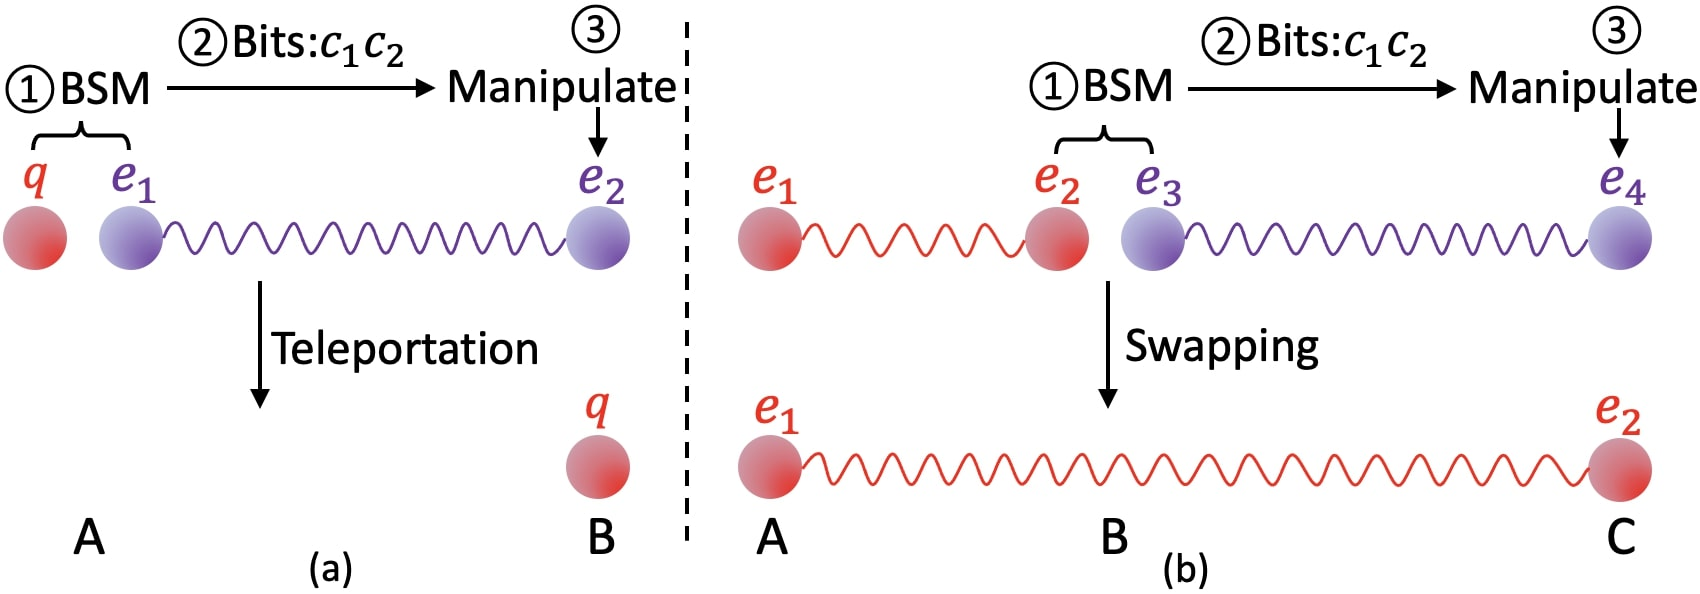
\includegraphics[width=0.8\textwidth]{chapters/tqe/figures/teleportation_swapping.jpg}
    \caption{(a)  Teleportation of $\ket{q}$ from $A$ to $B$, while consuming an entangled pair $(e_1, e_2)$. (b) Entanglement swapping over the triplet of nodes $(A, B, C)$, which results in $A$'s qubit entangled with $C$'s qubit. This can be viewed as a teleportation of $e_2$ from node $B$ to $C$.}
  \label{fig:swapping_teleport_swap}
\end{figure}

\para{Entanglement Swapping (\es).} 
Entanglement swapping is an application of teleportation 
to generate \epss over remote nodes. See Fig. \ref{fig:swapping_teleport_swap} (b).
If $A$ and $B$ share an \eps  and $B$ teleports its qubit to $C$, then 
 $A$ and $C$ end up sharing an \eps. 
%%%%%%%%
More elaborately, let us assume that $A$ and $B$
share an \eps, and $B$ and $C$ share a separate \eps. 
Now, $B$ performs a  BSM 
on its two qubits and communicates the result to $C$ (teleporting its 
 qubit that is entangled with $A$ to $C$). When $C$ finishes the protocol, it has a qubit
that is entangled with $A$'s qubit. Thus, an entanglement swapping (\es)
 operation can be looked up as being performed over a triplet of nodes $(A, B, C)$ 
with \eps available 
at the 
two pairs of adjacent nodes $(A, B)$ and $(B,C)$; it results in an \eps over the pair
of nodes $(A, C)$. 

\para{Fidelity: Decoherence and Operations-Driven.}
Fidelity is a measure of how close a realized state is to the ideal. 
Fidelity of qubit decreases with time, due to interaction with the environment,
as well as gate operations (e.g., in \es). 
%%%%%%
Time-driven fidelity degradation is called \emph{decoherence}. 
To bound decoherence, we limit the aggregate time a qubit spends in a 
quantum memory before being consumed.
%%%%%%%%
With regards to operation-driven fidelity degradation, 
Briegel et al.~\cite{BreigelEtAl1998} give an expression 
that relates the fidelity of an \eps generated by \es 
to the fidelities of the operands,  in terms of the 
noise introduced by swap operations and the number of link \epss used. The order of the swap operations (i.e., the structure of the 
swapping tree) does not affect the fidelity. 
%%%%%%%%%%%%%%%
Thus, the operation-driven fidelity degradation of the final \eps 
generated by a swapping-tree $T$
can be controlled by limiting the number of leaves of $T$, assuming that
the link \epss have uniform fidelity (as in~\cite{delft-lp}).

Entanglement Purification~\cite[e.g.]{BreigelEtAl1998} and Quantum Error 
Correction~\cite[e.g.]{QEC} have been widely used to combat fidelity 
degradation.  
Our work focuses on optimally scheduling \es operations with constraints
on fidelity degradation, without purification or error correction.

\para{Quantum Memories.}
Multiple quantum memories have been recently proposed to 
bring \tqbl{quantum networks} into realization. 
Types of quantum memories that support BSM measurements and gate unitary operations, and probably have a long decoherence time can be used in quantum communications.
Most of them are matter-based 
which have photonic interface to produce matter-matter entanglement 
over two neighboring nodes (see below).
%%%%%%%%%%
At a high-level, there are three different quantum memory platforms: quantum dots, trapped atoms or ions, and colour centers in diamond. 
%%%%%%%%%%%
Each has its own physical characteristics and applications. 
While quantum dots have the ability to process quantum information very fast, 
they exhibit a very low decoherence time among 
others~\cite{press2010ultrafast, wang2019towards}. 
To overcome the low efficiency of single atom-photon coupling process, 
atomic ensemble schemes have been proposed~\cite{dlcz} where along with dynamic decoupling and cooling techniques, decoherence times of a few seconds have been achieved~\cite{sagi10, vetsch10, deutsch10}.
%%%%%%
For trapped ion memories, decoherence times from several minutes to few hours have been demonstrated~\cite{ionqmemory05, ionqmemory21}.
%%%%%%%%%%%%%%%%%%%%%%%%%
To further 
increase the entanglement generation rate,~\cite{bhaskar2020experimental} proposes a way to use a single silicon–vacancy (SiV) 
colour center in diamond to perform asynchronous photonic BSM at 
the node located in the middle of two adjacent quantum nodes.

\subsection{Generating Entanglement Pairs (\epss)}
\label{sec:swapping_eps}

As described above, teleportation, which is the only viable means of transferring quantum states over long distances, requires an a priori distribution of \epss. 
Thus,   we need efficient mechanisms to  establish \epss across remote QN nodes; 
this is the goal of our 
work.
%\footnote{\blue{One could also do successive {\em teleportation} one-hop at a time, but this is conceptually equivalent to first establishing an a priori \eps between the remote nodes via a left-deep/right-deep swapping tree over local \eps's and then doing the teleportation.}}
%%%%%%%%%%%%%
Below, we start with describing how \epss are generated between adjacent
(i.e., one-hop away) nodes, and 
then discuss how \epss across a pair of remote nodes can be established 
via \ess. 


\para{Generating \eps over Adjacent Nodes.} 
The physical realization of qubits 
determines the technique used for sharing EPs between adjacent nodes. 
The \emph{heralded entanglement} process~\cite{sigcomm20, caleffi} to 
generate an atom-atom \eps between adjacent nodes $A$ and $B$
is as follows:
%entails each node generating an atom-photon entangled pair, 
%followed by
%an \es operation (optical BSM) which entangles the two atoms.} 
\begin{enumerate}
    \item 
Generate an entangled pair of atom and a telecom-wavelength photon at node $A$
and $B$.  
%; this is essentially done by exciting atoms (Rubidium (Rb) isotopes) by laser pulses. 
Qubits at each node are generally realized in an atomic form
%that is amenable 
for longer-term storage, while photonic qubits are used for transmission.
%The telecom-wavelength photons are well-suited for transmission over an optical fiber, while the atoms are better suited for memory storage.

\item 
Once an atom-photon entanglement is locally generated
at each node (at the same time), 
the telecom-photons are then transmitted over an optical fiber to a photon-photon/optical BSM device $C$ located in the middle of 
$A$ and $B$ so that the photons arrive at $C$ 
at the same time.

\item 
The device $C$ performs a BSM over the photons, 
and transmits the classical result to $A$ or $B$ to complete \es.
\end{enumerate}
%%%%%%
Other entanglement generation processes have been 
proposed~\cite{muralidharan2016optimal}; %our evaluation 
%technical development 
%uses the heralded entanglement;
%generation process as in~\cite{sigcomm20, caleffi}; 
%however,
our techniques themselves are independent of how the link \eps are generated.

%To d \eps between adjacent nodes, we can directly generate an \eps at one node and  transmit one qubit of the \eps to the neighbor, with repeated generation and transmission in case of a loss/error.
%%%%%%%%%%%%%%

%%%%=====>
%%%     X-Y entanglement to be generated at node.
%%%%    X will be stored and we can do BSM on them.
%%%%%   Y will be transmitted. 
%%%%    There are memory platform that enable the above scheme of EP generation over adjacent nodes. And, has two "good" parameters: decoherence time (a few seconds), effective excitation rate (20 microseconds).











\para{Generating \eps between Remote Nodes.} 
Now, \eps between non-adjacent nodes connected by a path in the network 
can be established by 
performing a sequence of \ess at 
intermediate nodes; this requires an a priori \eps over 
each of the adjacent pairs of nodes in the path.
%%%%%%%%%%
For example, consider a path of nodes $x_0, x_1, x_2, x_3, x_4, x_5$, with an \eps 
between every pair of adjacent nodes $(x_i, x_{i+1})$. Thus, each node $x_i$
($1 \leq i \leq 4$) has two qubits, one of which is entangled with $x_{i-1}$ 
and the other with
$x_{i+1}$. Nodes $x_0$ and $x_5$ have only one qubit each.
%%%%%%%%%%%%%%%%%
To establish an \eps 
between $x_0$ and $x_5$, we can perform a sequence of entanglement
swappings (\ess) as shown in Fig.~\ref{fig:swapping_tree}. 
\eat{over the following triplet of nodes:
(i) \es over  $(x_1, x_2, x_3)$ to yield an \eps over $(x_1, x_3)$,
(ii) \es over  $(x_1, x_3, x_4)$ to yield an \eps over $(x_1, x_4)$,
(iii) \es over  $(x_1, x_4, x_5)$ to yield an \eps over $(x_1, x_5)$,
(iv) \es over  $(x_0, x_1, x_5)$ to yield an \eps over $(x_0, x_5)$.}
%%%%%%%%%%%%%%%%%%%%%
Similarly, the sequence of \es over the following triplets would also 
work: $(x_2, x_3, x_4)$, $(x_2, x_4, x_5)$, $(x_0, x_1, x_2)$, 
$(x_0, x_2, x_5)$. 
\eat{Note that some of the above \es can happen \ul{in parallel}, e.g.,
$(x_0, x_1, x_2)$ and $(x_2, x_3, x_4)$ 
can happen 
in parallel, as 
they are over separate sets of qubits.}
%%%%%%%%%%%%%%%%%%%%%%%%%%%%%%%%%%

\begin{figure}[h]
    \centering
    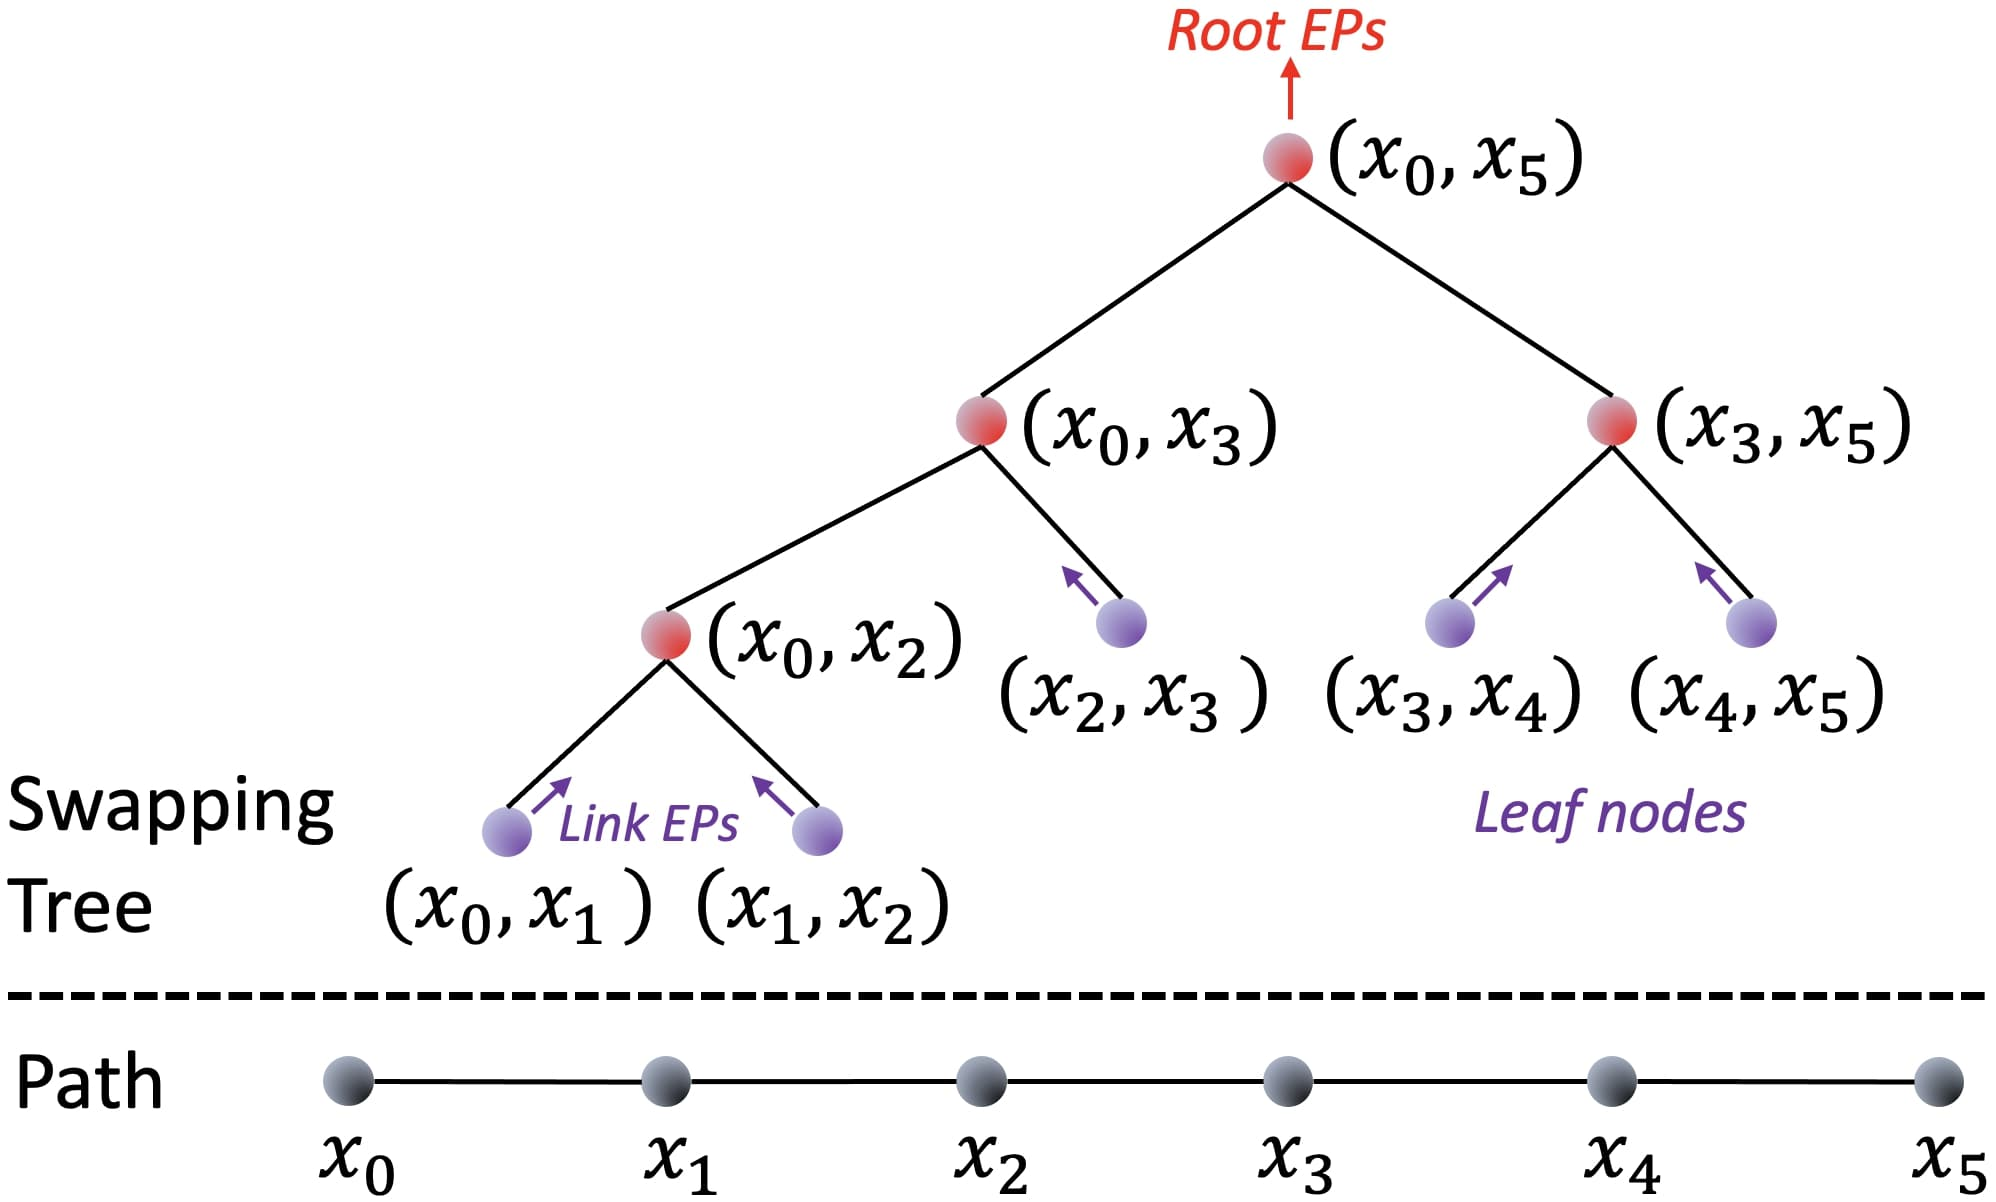
\includegraphics[width=0.75\textwidth]{chapters/tqe/figures/swapping_tree.jpg}
    \caption{A swapping tree over a path. The leaves of the tree are the path-links, which generate link-\epss continuously.}
\label{fig:swapping_tree}
\end{figure}

\para{Swapping Trees.}
In general, given a path $P = s \leadsto d$ from $s$ to $d$, 
any complete binary tree (called a \textit{swapping tree}) over 
the ordered links in $P$ gives a way to generate an \eps over $(s, d)$.
%%%%%%%%%%%%
Each vertex in the tree corresponds to a pair of network nodes in $P$, 
with each leaf representing a link in $P$. 
%%%%%%%%%%%%%%
Every pair of siblings $(A, B)$ and $(B, C)$ perform an \es over 
$(A,B,C)$  to yield an \eps over $(A,C)$---their parent.
See Fig.~\ref{fig:swapping_tree}. 
\emph{Note that subtrees of a swapping tree execute in parallel.}
%%%%%%%%%%%%%%%%%%%%%%%%%%
Different swapping trees over the same path $P$ can have different performance characteristics, as discussed later (see Fig.~\ref{fig:swapping_non-balance}).
%In particular, when a swapping tree is used to continuously 
%generate \epss over the root pair, using \epss being generated continuously at
%the links/leaves, different swapping trees can incur very different expected 
%latency in generating \epss, as discussed below. 

\softpara{Expected Generation Latency/Rate of \epss.}
In general, our goal is to continuously generate \epss at some rate using 
a swapping tree, using continuously generated \epss at the leaves. 
The stochastic nature 
of %the physical mechanisms underlying 
\es operations
means that an \eps at the tree's root will be successfully 
generated only after many failed attempts and hence significant latency.
We refer to this latency as the \textit{generation latency} of the \eps at the 
root, and in short, just the generation latency of the tree. 
{\eps generation rate} 
is the inverse of its generation latency. Whenever we refer to generation 
latency/rate, we implicitly mean \textit{expected} generation latency/rate. 

\para{Two Generation Protocols: \os and \wt}
When a swapping tree is used to (continuously) generate \epss, there are two 
fundamentally different generation protocols~\cite{gisin,tittel-08}. 

\begin{itemize}
\item \textit{\os Protocol.}  
%In the \os protocol, an \eps (i.e., the corresponding qubits) is \blue{not stored in the memory} to wait for another \eps to be generated, as in the \wt protocol. 
In this model, all the underlying processes, including link \eps generations and atomic
BSMs are synchronized. If all of them succeed then the end-to-end \eps is generated.
%almost instantaneously. 
If \textit{any} of the underlying processes fail,
then all the generated \epss are discarded and the
whole process starts again from scratch (from generation of \eps at links).
In the \os protocol, all swapping trees over a given path $P$
incur the same generation latency---thus, here, the
goal is to select an optimal path $P$ (as in~\cite{sigcomm20,delft-lp}).  \eat{Since all underlying processes have to succeed simultaneously to generate an end-to-end EP, these protocols are inherently exponential in the number of nodes in $P$.} 

\item \textit{\wt Protocol.} In \wt protocol, a qubit of an \eps 
may wait (in a quantum memory) for its counterpart to become available so that an \es operation can be performed. 
Using such storage, we preclude discarding successfully generated \epss, and 
thus, reduce the overall latency in generation of a root-level \eps. 
E.g., let  $(A,B)$ and $(B,C)$ be two siblings in a swapping tree and \eps for $(A,B)$ is generated first. Then, \eps $(A,B)$ may wait for the \eps $(B,C)$ to be successfully generated. 
Once the \eps $(B,C)$ is generated, the \es operation
is done over the triplet $(A, B, C)$ to generate the \eps $(A,C)$. 
If the \eps $(A,B)$ waits beyond a certain threshold, then it may decohere.   
\end{itemize}

\softpara{Hardware Requirement Differences.}
\os protocols can generate \epss without quantum memories in a relay fashion if 
the EP generation among adjacent nodes can be tightly synchronized. In contrast,
\wt protocols benefit from memories with good coherence times (\S\ref{sec:swapping_eval}).

\para{Why \wt's Entanglement Generation Rate is Never Worse.} 
The focus of the \os protocol is to avoid qubit decoherence  
due to storage. But it results in very low generation rates
due to a very-low probability of \textit{all} the underlying 
processes succeeding at the same time. 
%%%%%%%%%%%%%%%%%%%%%%%%%%
However, since qubit coherence times are 
typically higher than the link-generation latencies\footnote{Link generation latencies 
for 5 to 100km links range from about 3 to 350 milliseconds
for typical network parameters~\cite{caleffi}, while coherence times of few
seconds is very realistic (coherence times of several seconds~\cite{Longdell-2005,Fraval-2005} have been shown 
long ago, and more recently, 
even coherence times of several minutes~\cite{dec-13,dec-14} to a few hours~\cite{dec-15,dec-2021} 
have been demonstrated.},
an appropriately designed \wt protocol will always 
yield better generation rates \textit{without significantly compromising the fidelity} %(see Theorem~\ref{thm:swapping_os-wt}). 
The key is to bound the waiting time to limit decoherence
as desired; e.g., in our protocol, we restrict to trees with high expected 
fidelities (\S\ref{sec:swapping_problem}), and discard qubits that
"age" beyond a threshold.
%%%%%%%%%%%
\bleu{Both protocols use the same number of quantum memories (2 per node), though the \wt protocols will benefit from low-decoherence memories; other hardware requirements 
also remain the same.}

\eat{We note that both protocols require the \red{same number of quantum memories}---two 
per node---but \wt protocol benefit from low-decoherence memories; 
other hardware 
requirements are also same.} 
%%%%%%%%%%%%%%%

% \begin{theorem}
% Consider a quantum network, a path $P$, a swapping-tree $T$ over $P$, a \os protocol $X$, and a \wt protocol $Y$. Protocol $Y$ discards qubits that age (stay in  memory) beyond a certain threshold $\tau$ (presumably, equal to the coherence time). 
% We claim that $Y$'s \eps generation rate will at least be that of $X$, 
% irrespective of $\tau$ and $T$ (as long as it is over $P$), 
% while ensuring that \epss generated by $Y$ are formed by non-decohered qubits and the operation-driven fidelity degradation of $Y$ \epss is same as $X$.
% \label{thm:swapping_os-wt}
% \end{theorem}

% \section{Proof of Theorem~\ref{thm:swapping_os-wt}}
% \label{app:swapping_os-wt}
% \section{PROOF OF THEOREM~\ref{thm:os-wt}}
% \label{app:os-wt}

% \para{Proof (sketch):} 
% We provide a main intuition behind the claim in Theorem~\ref{thm:swapping_os-wt}.
% The key claim is that at any instant the \os protocol generates an \eps,
% the \wt protocol will also be able to generate an \eps.
% Consider an instant $t$ in time when the \os protocol $X$ generates an 
% \eps, as
% a result of all the underlying processes succeeding at time $t$. 
% Right before time $t$, consider the state of the \epss in the swapping-tree $T$ of the \wt 
% protocol $Y$: Essentially, some of the nodes in $T$ have (generated) 
% \epss that are waiting for their sibling \eps to be generated; note that these generated \epss have not aged yet, else they would have been already discarded by $Y$. 
% Now, at time $t$, during $X$'s execution, all the underlying processes succeed instantly---it is easy to see that in the protocol $Y$ too, all the un-generated \eps would now be generated instantly\footnote{Here, we have implicitly assumed that if $n$ BSM operations succeed in $X$ protocol at some instant $t$, then at the same instant, $n$ BSM operations anywhere in $Y$ will also succeed.}---yielding a full \eps at the root (using qubits that have not aged beyond the threshold).
% Finally, since the number of operations in $T$ is the same as the number of BSM operations incurred by $X$ to generate an \eps, the fidelity degradation due to operations is the same in both the protocols.

% The above theorem suggests that \wt approach is always a better 
% performing approach, 
% irrespective of the decoherence time/limitations.
% See proof in Appendix~\ref{app:swapping_os-wt}. 



%In our simulation results, for our settings, \epss generated by our \wt protocol have fidelities comparable to that of the \os protocol; note that the \epss generated by the \os protocol also incur fidelity degradation due to the unavoidable \es operations.
%Note that the \wt approach naturally degenerates to the \os approach when
%the waiting is bounded to zero---as in such as case, all swapping trees over
%a given path would have equal 

%\red{Can the \os model work with no memories? i.e., with "relays"? See Gisin paper.}



